% Figure blocks for the paper. Rounded blue boxes are steps, orange boxes are model calls,
% green boxes are checks with no model, slanted yellow boxes are data, purple cylinders are
% stores and red boxes are findings. Each PDF builds from its .tex with pdflatex.

\begin{figure*}[t]
  \centering
  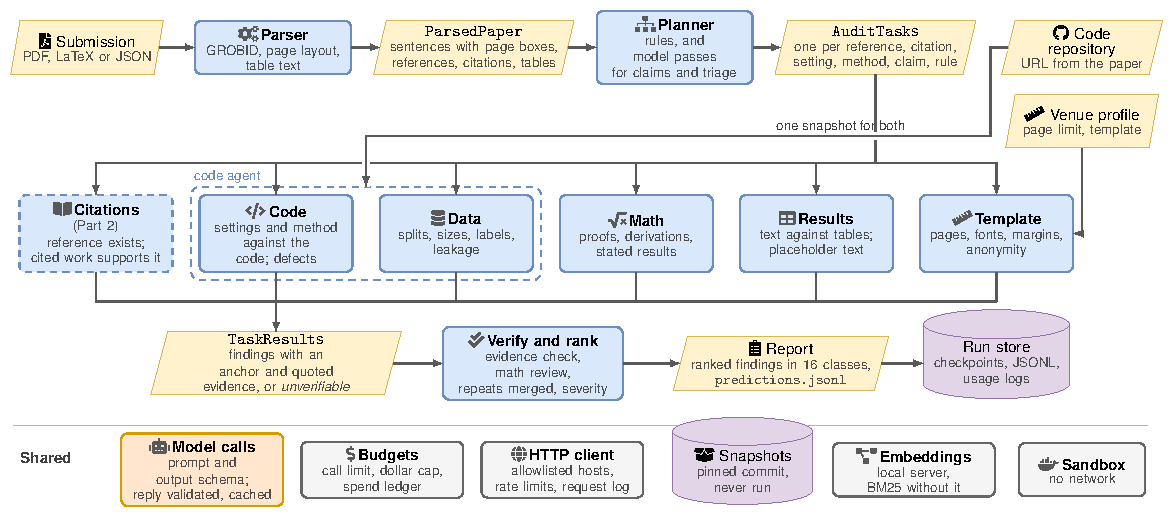
\includegraphics[width=\textwidth]{figures/system.pdf}
  \caption{The auditor. The parser turns the submission into sentences with page boxes. The
  planner makes one task per reference, citation, stated setting, method, claim and venue rule.
  Each task goes to the checker for its kind; the code and data checkers share one snapshot of
  the repository. Every finding names its sentence or code lines and quotes its evidence. The
  citation checker is built in Part 2.}
  \label{fig:system}
\end{figure*}

\begin{figure*}[t]
  \centering
  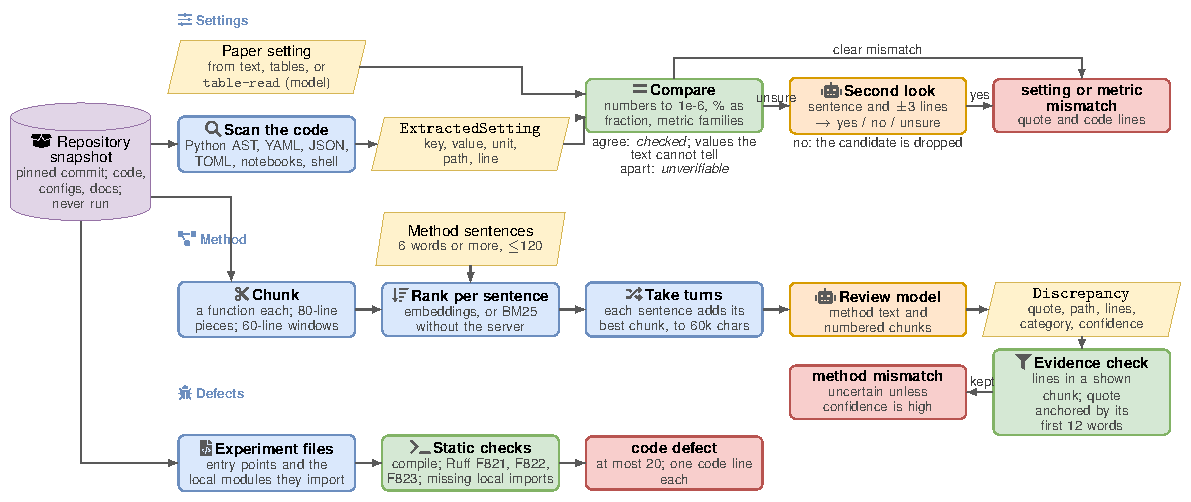
\includegraphics[width=\textwidth]{figures/code.pdf}
  \caption{The code checker. A stated setting is compared with every value the static scanners
  find, and a model reads the code only when the comparison cannot decide. For the method, each
  sentence ranks the code chunks, and the sentences take turns filling a 60k-character budget.
  The checker keeps a reported discrepancy only if its lines were shown and its quote is in the
  paper.}
  \label{fig:code}
\end{figure*}

\begin{figure*}[t]
  \centering
  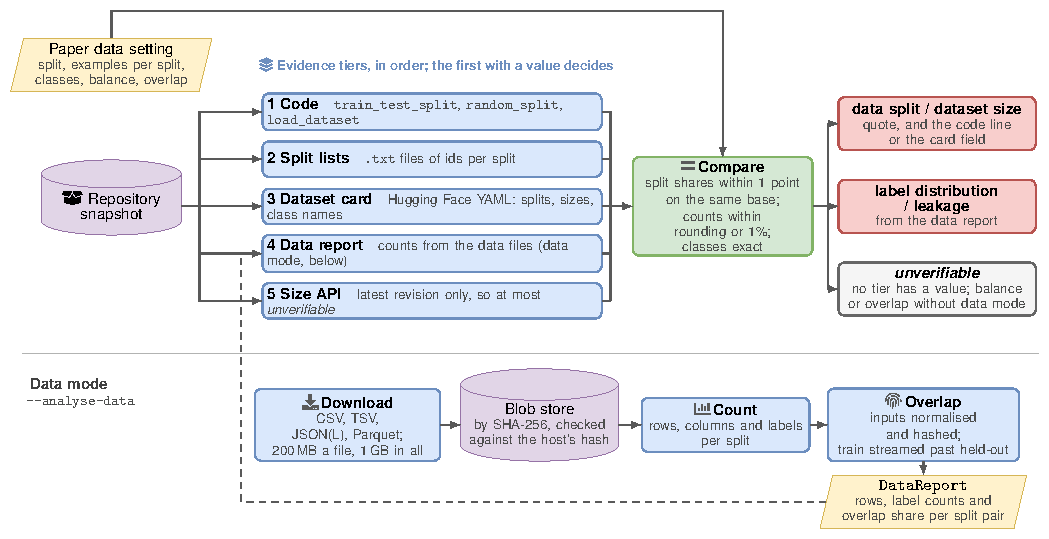
\includegraphics[width=\textwidth]{figures/data.pdf}
  \caption{The data checker. Stated splits, sizes, classes and overlap are compared with the
  first source that gives a value, in the order shown. Class balance and train/test overlap
  need the data files, which are downloaded and counted only in data mode. No step calls a
  model.}
  \label{fig:data}
\end{figure*}

\begin{figure*}[t]
  \centering
  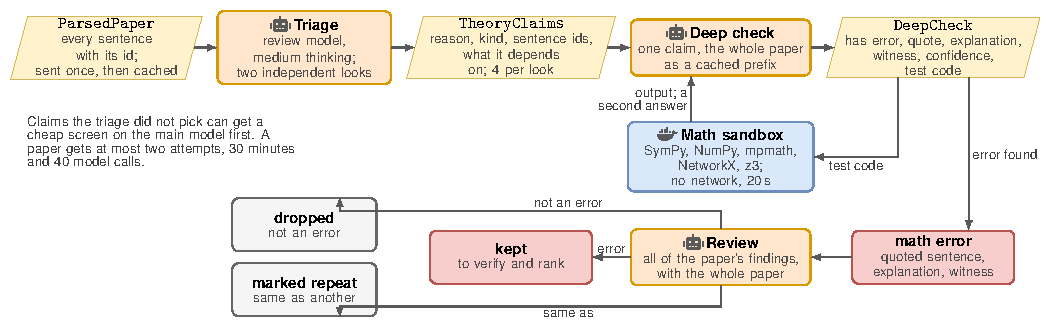
\includegraphics[width=\textwidth]{figures/math.pdf}
  \caption{The math checker. Two triage calls each pick up to four claims to check. A deep check
  reads one claim with the whole paper, which is sent once and cached, and may write a test
  that runs in the sandbox before it answers again. A last call reads all of the paper's
  findings together and drops the refuted ones.}
  \label{fig:math}
\end{figure*}

\begin{figure*}[t]
  \centering
  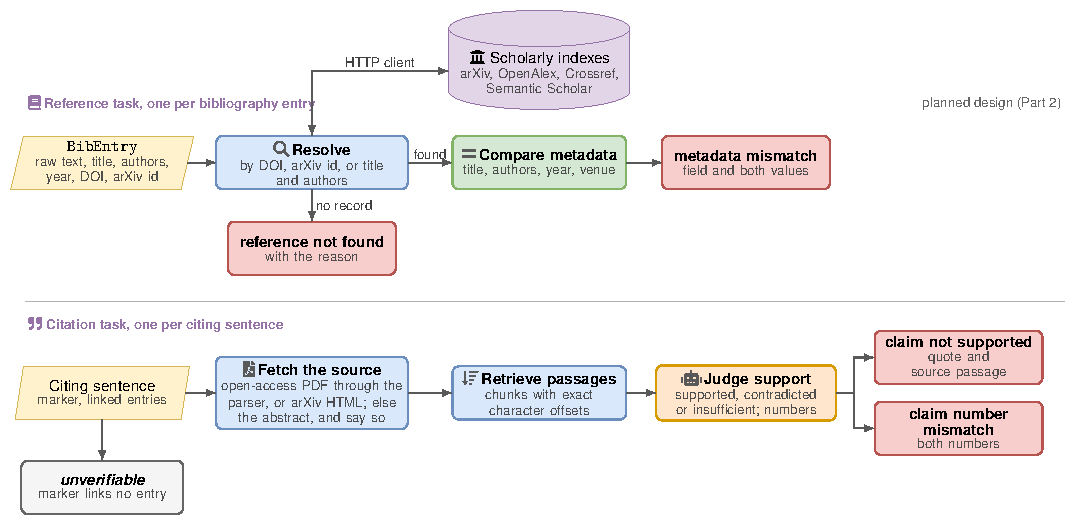
\includegraphics[width=\textwidth]{figures/citation.pdf}
  \caption{The citation checker as planned for Part 2. It looks each reference up by DOI, arXiv id
  or title. It judges a citing sentence against passages of the cited work, or against the
  abstract when the full text is closed. A marker that links no entry is reported as
  unverifiable.}
  \label{fig:citation}
\end{figure*}
